%第3章


\section{要求定義}


商品識別システムがどのように機能すべきかという振る舞いと,その外部環境を表すためにユースケース図を作成した.以下に図\ref{usecase1}を載せる.

\begin{figure}[htbp]
\centering
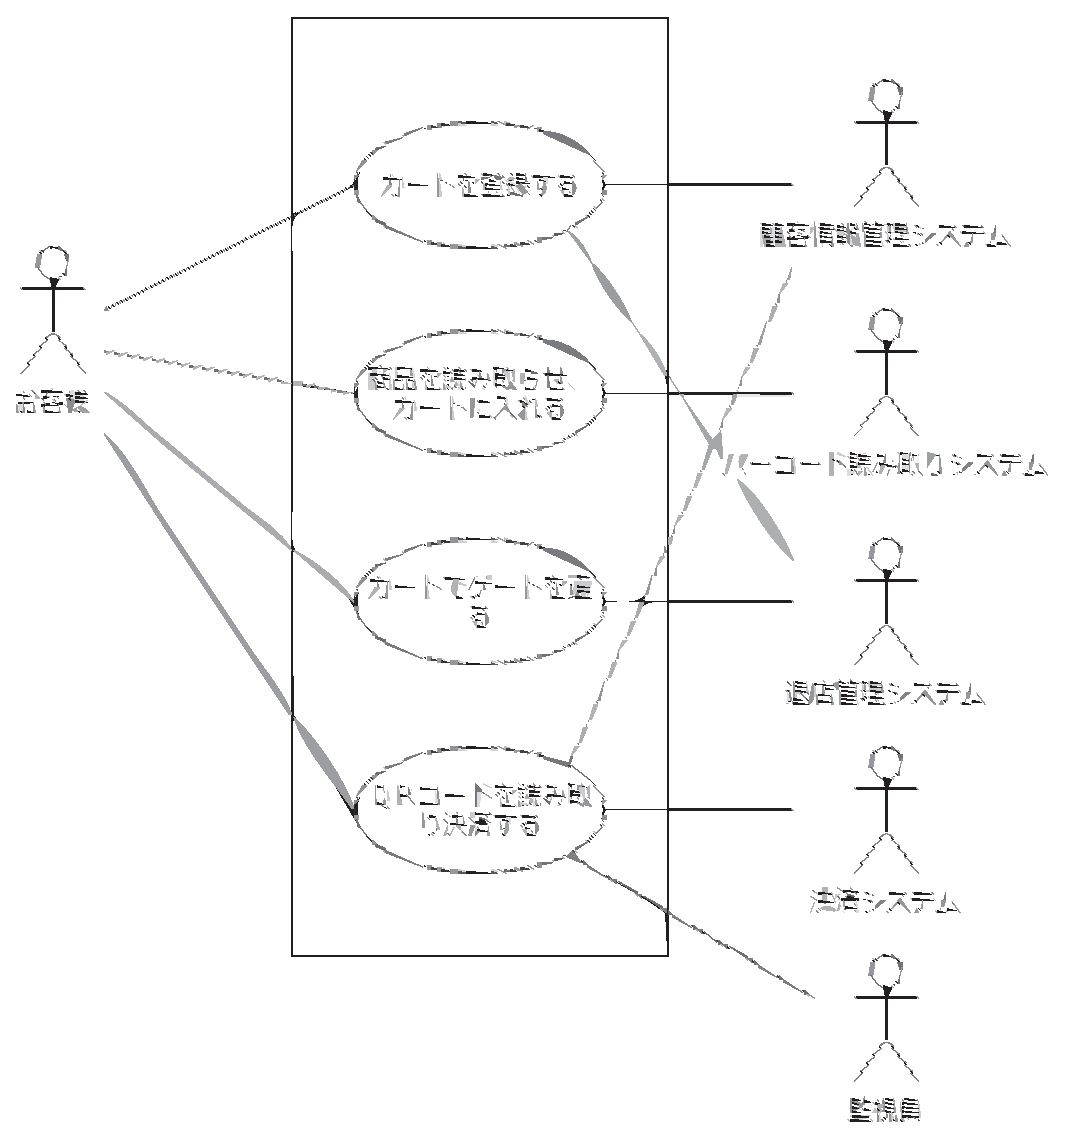
\includegraphics{./picture/usecase1.eps}
\caption{システムのユースケース図(1)}
\label{usecase1}
\end{figure}

\begin{figure}[htbp]
\centering
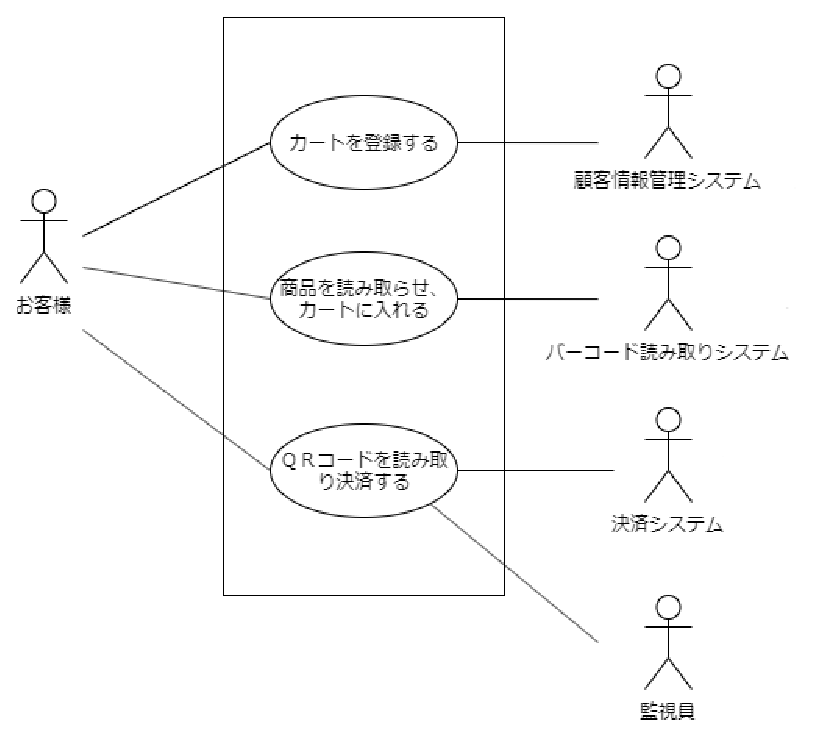
\includegraphics[width = 15cm]{./picture/usecase2.eps}
\caption{システムのユースケース図(2)}
\label{usecase2}
\end{figure}

\begin{figure}[htbp]
\centering
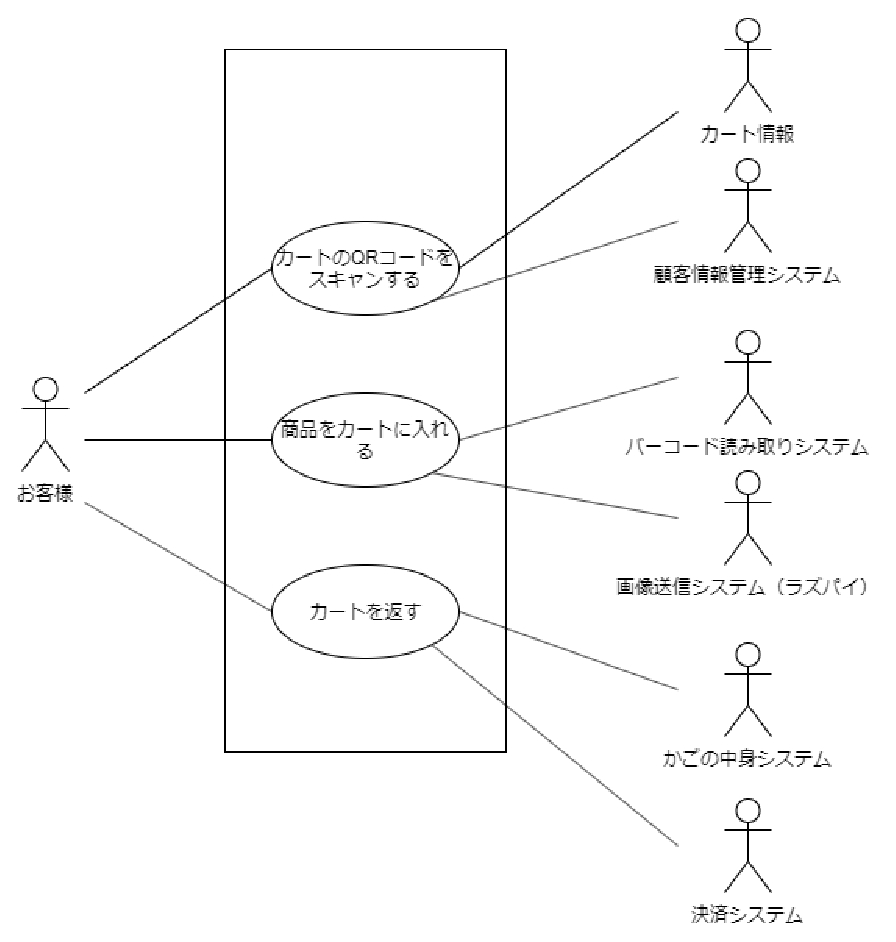
\includegraphics{./picture/usecase3.eps}
\caption{システムのユースケース図(3)}
\label{usecase3}
\end{figure}

\begin{figure}[htbp]
\centering
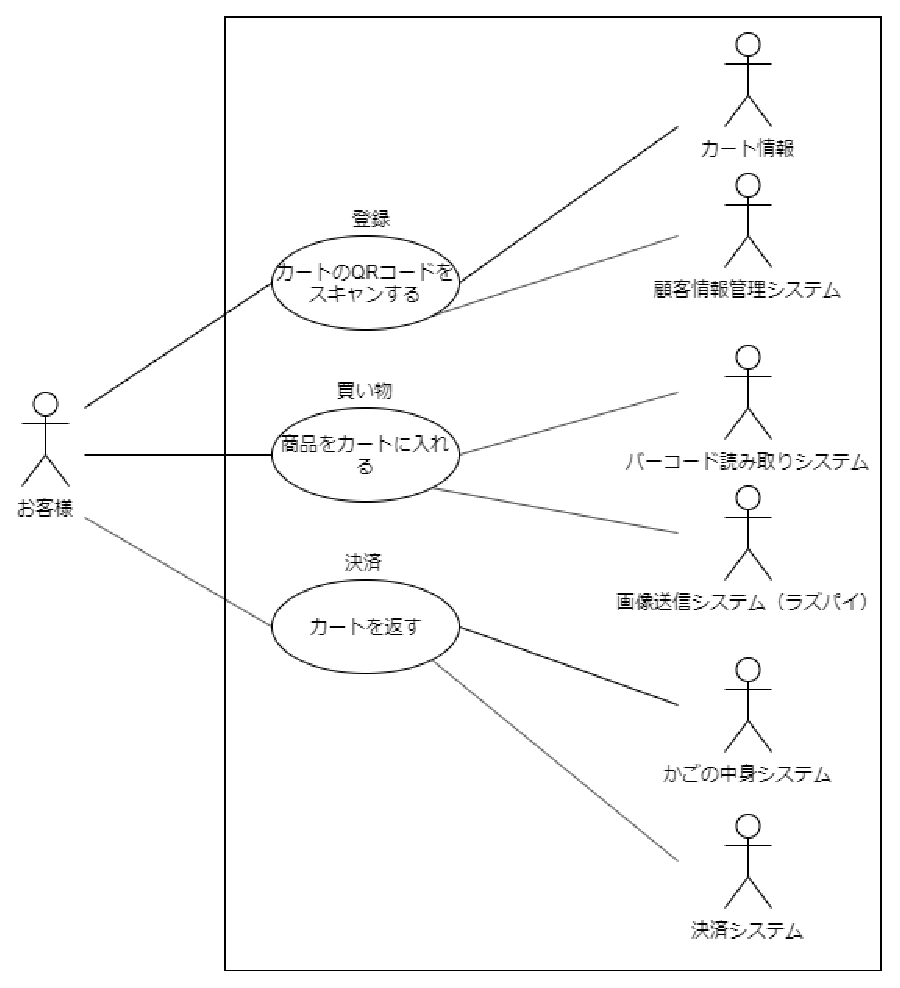
\includegraphics[width = 15cm]{./picture/usecase_qr.eps}
\caption{QRコードを用いたシステムのユースケース図}
\label{usecase_qr}
\end{figure}

\begin{figure}[htbp]
\centering
\includegraphics[width = 15cm]{./picture/usecase_ic.eps}
\caption{ICタグを用いたシステムのユースケース図}
\label{usecase_ic}
\end{figure}


